\chapter{View}\label{cap:view}
In questo capitolo si tratterà la componente \textit{View} del sistema realizzato. In tale livello è stata implementata l'interfaccia grafica che consente una semplice e rapida interazione con lo Spider, in particolare le interfaccie progettate sono di tipo:
\begin{description}
\item[Desktop Application:] realizzata puramente per utilizzo di tipo desktop;
\item[Web Application:] per un utilizzo di tipo web, ovvero tramite browser.
\end{description}
Si è deciso di intraprendere questa strada per rendere il più user-friendly possibile la nostra applicazione, infatti, grazie alla capacità di gestione delle interazioni desktop$\Leftrightarrow$web che ha il Java, è risultato molto semplice comunicare i risultati delle ricerche da desktopApp alla webApp. In questo modo si è realizzata una interfaccia molto simile ai motori di ricerca che vengono utilizzati quotidianamente sul web. Un esempio pratico di quanto esposto può essere il seguente:
\begin{enumerate}
\item si inseriscono il task e la query;
\item si avvia lo spidering;
\item ad intervalli viene effettuata una ricerca della query specificata;
\item i risultati vengono visualizzati su una pagina web (in particolare jsp);
\item l'utente è in grado di navigare i risultati per pagine, come fossero i risultati di un motore di ricerca stile Google$^{TM}$.
\end{enumerate}
Un esempio più dettagliato lo si può trovare nel capitolo \ref{cap:example}.
\section{Desktop Application}
\begin{figure}[htb]
\begin{center}
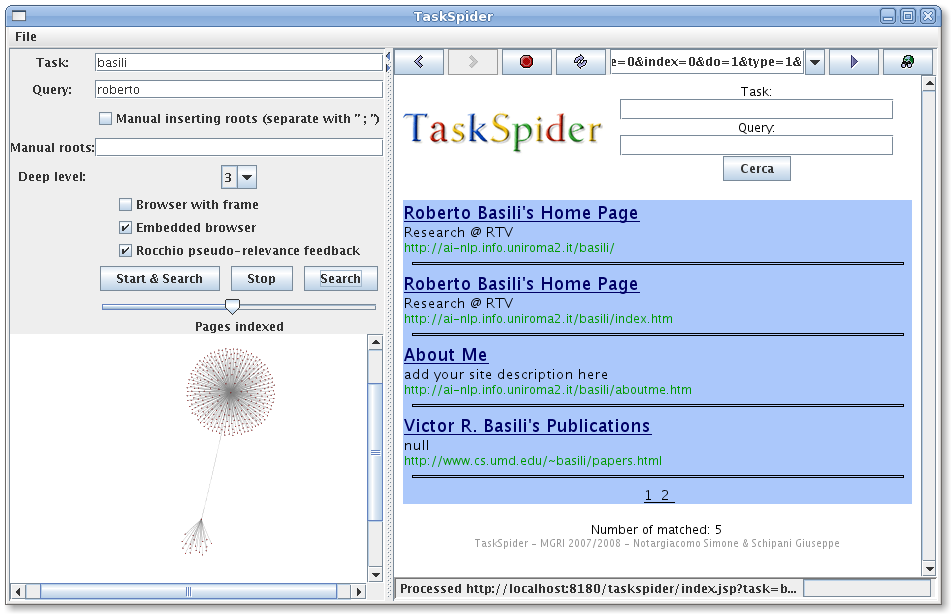
\includegraphics[scale=0.4]{etc/taskspider.png}
\caption{Desktop Application}
\label{desktopApp}
\end{center}
\end{figure}
L'interfaccia grafica realizzata per desktop è formata da:
\begin{itemize}
\item alcuni campi per l'immissione del task e della query;
\item campi di opzioni per scegliere le modalità di ricerca, visualizzazione ed altro;
\item pulsanti per avviare lo spidering e la ricerca;
\item un grafo rappresentante la rete delle pagine web filtrate;
\item un browser web per visualizzare i risultati della ricerca e navigarli.
\end{itemize}
\section{Web Application}
\begin{figure}[htb]
\begin{center}
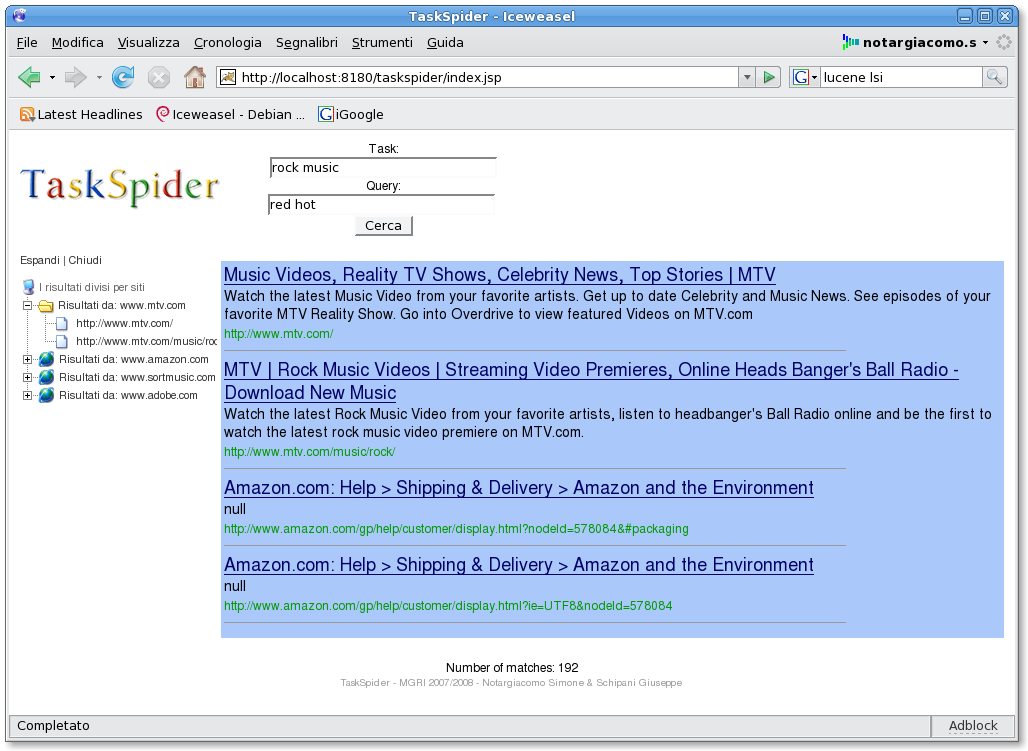
\includegraphics[scale=0.35]{etc/webApp.png}
\caption{Web Application}
\label{webApp}
\end{center}
\end{figure}
Si è deciso di realizzare una pagina web in grado di effettuare delle ricerca sugli indici e in grado di rappresentare i risultati sotto varie forme. In particolare è stata implementata considerando due modalità di utilizzo:
\paragraph{Solo ricerca}
Questo caso si ha quando si accede alla pagina direttamente dal browser, senza passare argomenti tramite barra degli indirizzi. Questa modalità consente di effettuare una ricerca sugli indici già memorizzati sul sistema; la ricerca può essere avviata utilizzando i campi Task e Query appositamente creati. I risultati possono essere visualizzati sia come un semplice elenco di indirizzi oppure anche con un albero che riunisce i risultati per dominio.
\paragraph{Spidering e Ricerca}
Questo secondo caso si verifica quando la pagina web viene acceduta dalla Desktop Application, la quale effettua lo spidering ed in seguito richiama la pagina. E' opportuno specificare che la pagina, in realtà si comporta sempre nello stesso modo, ovvero esegue una ricerca sull'indice richiesto. C'è un unica differenza rispetto al caso precedente, ovvero che nella modalità attuale tutti i dati per effettuare la ricerca vengono passati tramite barra degli indirizzi (\var{QueryString}); inoltre l'albero dei risultati per domino è opzionale.